\documentclass[12pt]{article}
\usepackage[utf8]{inputenc}
\usepackage[finnish]{babel}
\usepackage{graphicx}
\usepackage{float}
\usepackage{hyperref}
\title{Aineopintojen harjoitustyö: Tietokantasovellus\\Dokumentaatio}
\author{Sandra Luhtaniemi}
\begin{document}
\maketitle
\section{Johdanto}
Harjoitustyön aiheena on lankatietokanta. Tietokannan tarkoitus on tarjota käyttäjälleen väline, jolla pitää kirjaa omistamistaan eri käsityölangoista, näiden materiaalista, paksuudesta ja määrästä. Käyttäjä voi esimerkiksi kohdatessaan kiinnostavan neuleohjeen, hakea ohjeessa mainitun langan ominaisuuksien perusteella tietokannasta ne langat, joilla työ olisi mahdollista toteuttaa, sekä tarkistaa, onko hänellä sitä riittävä määrä. Käyttäjä voi myös muilla perusteilla etsiä tietokannasta lankoja, esimerkiksi vaikkapa kaikki sukkalangat. Käyttäjä voi lisätä tietokantaan uudet lankahankintansa, poistaa langan, tai päivittää sen määrän käytettyään jotakin lankaa. Järjestelmän tavoitteena on helpottaa käsitöiden suunnittelua ja vähentää turhia lankahankintoja.
\\ \ \\
Järjestelmä käyttää PostgreSQL-tietokantaa, se toteutetaan php-ohjelmointikielellä, ja se pyörii Tietojenkäsittelytieteen laitoksen users-palvelimella Apache-palvelimen alla. 
\\
\ \\
\textbf{Käyttötapaukset}\\ 
Käyttäjäryhmät:\\
Tietokannalla on vain yksi käyttäjäryhmä. Käyttäjän on rekisteröidyttävä päästäkseen käyttämään tietokantaa. Tämän jälkeen hän voi lisätä tietokantaan lankojaan ja tarkastella tai suorittaa hakuja omistamistaan langoista. 
\\ \ \\
Käyttäjän käyttötapaukset\\
Rekisteröityminen: Käyttäjä luo ensimmäisellä käyttökerralla itselleen käyttäjätunnuksen ja salasanan.
\\ \ \\
Langan lisääminen: Käyttäjä lisää tietokantaan uuden langan
\\ \ \\
Langan poistaminen: Käyttäjä poistaa tietokannasta langan, jonka on käyttänyt loppuun.
\\ \ \\
Langan määrän päivittäminen: Käyttäjä päivittää langan määrän käytettyään siitä osan.
\\ \ \\
Lankojen tarkastelu: Käyttäjä tarkastelee listaa omistamistaan langoista.
\\ \ \\
Haku ominaisuuden perusteella: Käyttäjä hakee tietokannasta kaikki jollakin ominaisuudella varustetut langat.
\\ \ \\
Omien tietojen muuttaminen: Käyttäjä muuttaa omia tietojaan, esimerkiksi salasanaansa tai nimeään.
\\ \ \\
\begin{figure}[H]
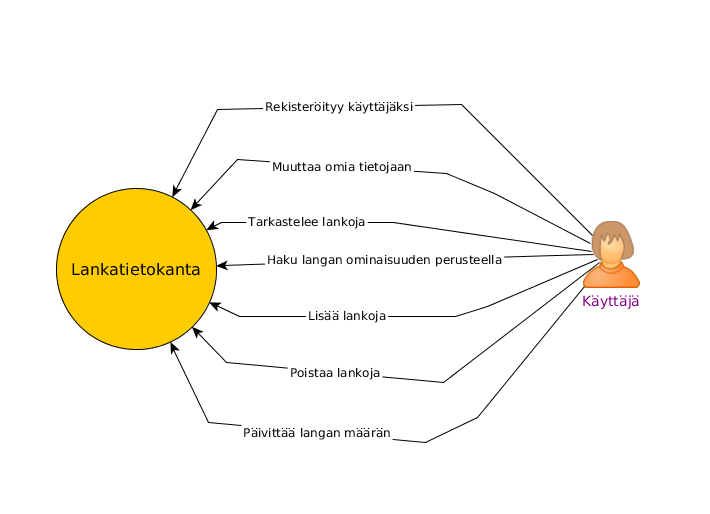
\includegraphics[scale=0.5]{sidosryhmakaavio.png}
\caption{Sidosryhmäkaavio}
\end{figure}
\begin{figure}[H]
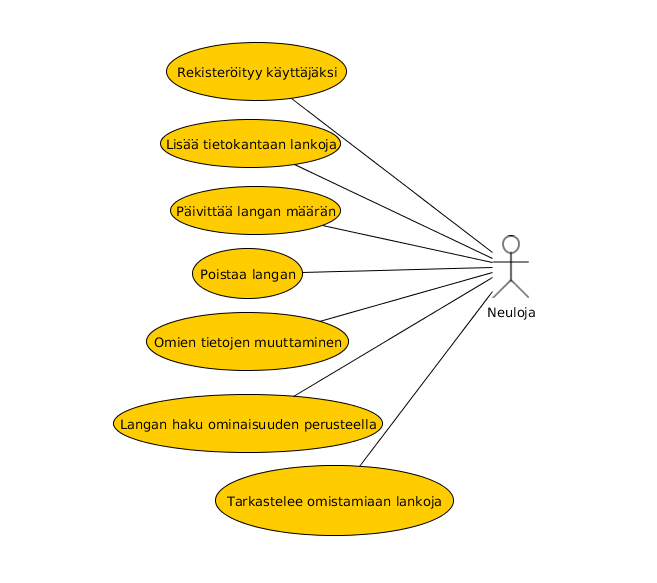
\includegraphics[scale=0.5]{kayttotapaukset.png}
\caption{Käyttötapauskaavio}
\end{figure}

\section{Käyttöliittymän suunnittelu}
Tietokohde: Yarn\\
\begin{tabular}[H]{|c|c|c|}
\hline
Attribuutti & Arvojoukko & Kuvailu \\
\hline
yarnname & Merkkijono & Langan kauppanimi \\
\hline
yarnmanu & Kokonaisluku & Langan valmistajan id-luku\\
\hline
nsrmin & Kokonaisluku & Puikkosuosituksen alaraja kerrottuna 10:llä \\
\hline
nsrmax & Kokonaisluku & puikkosuosituksen yläraja kerrottuna 10:llä \\
\hline
lpg & Kokonaisluku & Sadan gramman sisältämä metrimäärä \\
\hline  
\end{tabular}
\\
Lanka, jolla on jokin puikkosuositus, eli valmistajan antama suositus siitä minkä kokoisilla puikoilla sitä kannattaa neuloa. Puikkosuosituksella on yleensä alaraja ja yläraja, sillä käsiala voi vaihdella neulojasta riippuen. Langalle on ilmoitettu myös metrimäärä, joka sisältyy sataan grammaan, sillä sen avulla voi arvioida langan riittoisuutta.
\ \\ \ \\
Tietokohde: manu\\
\begin{tabular}{|c|c|c|}
\hline
Attribuutti & Arvojoukko & Kuvailu \\
\hline
manuname & Merkkijono & Valmistajan nimi \\
\hline
\end{tabular}
\\
Langan valmistanut yritys.
\ \\ \ \\
Tietokohde:users\\
\begin{tabular}{|c|c|c|}
\hline
Attribuutti & Arvojoukko & Kuvailu \\
\hline
username & Merkkijono & Käyttäjän valitsema käyttäjätunnus\\
\hline
password & Merkkijono & Käyttäjän valitsema salasana\\
\hline   
\end{tabular}
\\
Tietokannan käyttäjä valitsee rekisteröityessään jonkin käyttäjätunnuksen ja salasanan. 
\ \\ \ \\
Tietokohde:attr\\
\begin{tabular}{|c|c|c|}
\hline
Attribuutti & Arvojoukko & Kuvailu \\
\hline
attrname & Merkkijono & langan ominaisuus, esim. väri tai materiaali\\
\hline   
\end{tabular}
\\
Langoilla on erilaisia ominaisuuksia, esimerkiksi väri, materiaali tai vaikkapa huopuvuus tai väriin liityvä erikoisominaisuus, kuten liukuvärjäys. Langalla voi olla useita attribuutteja, ja sama attribuutti voi liittyä useaan eri lankaan. 
\ \\ \ \\
Tietokohde: owns\\
\begin{tabular}{|c|c|c|}
\hline
Attribuutti & Arvojoukko & Kuvailu \\
\hline
amount & kokonaisluku & Kayttajan omistama määrä kyseistä lankaa\\
\hline  
\end{tabular}
\\
Tietokanta voi sisältää monia eri lankoja, mutta käyttäjällä ei välttämättä ole näitä kaikkia tai eri käyttäjillä on lankoja eri määrä. 
\section{Asennusohje}
Tiedostot kopioidaan paikkaan, missä niitä halutaan säilyttää. Tiedostoon lib/settings.php laitetaan asetukset, jolla voidaan muodostaa yhteys tietokantaan. Tietokantaan luodaan taulut ajamalla tiedosto sql/create\_tables.sql ja käyttäjä ajamalla tiedosto sql/init\_admin.sql. 
\section{Käynnistys- ja käyttöohje}
Tietokanta löytyy osoitteesta \href{http://aluhtani.users.cs.helsinki.fi/tsoha/login.php}{http://aluhtani.users.cs.helsinki.fi/tsoha/login.php}
\\
Kirjautumista ja toimintoja voi kokeilla käyttäjätunnuksella ja salasanalla: ``Anneli'' ja "asdf''.
\section{Järjestelmän yleisrakenne}
Tietokantasovellusta tehdessä on noudatettu MVC-mallia. Kontrollerit ovat juurikansiossa. Näkymät ja malliluokat ovat kansioissa views ja lib. Apukirjastot löytyvät myös kansiosta lib. Asetukset ovat tiedostossa settings.php. Ylläpidon sivuista vastaavissa tiedostoissa on admin-etuliite. Kaikki tiedostonimet on kirjoitettu pienellä. 
\section{Järjestelmän komponentit}
index.php\\
Siirtää käyttäjän sovelluksen sisäänkirjautumissivulle.\\
\ \\
login.php\\
Sisältää kentät sisäänkirjautumista varten. Tänne tulee myös linkki käyttäjäksi rekisteröitymistä varten.\\
\ \\
views/login.php\\
Sisältää Kirjautumissivun näkymän.\\
\ \\
logout.php\\
Kirjaa käyttäjän ulos.\\
\ \\
home.php\\
Sisäänkirjautuneen käyttäjän etusivu. Sisältää linkin omien lankojen tarkasteluun. Admin-käyttäjälle näkyy myös linkki hallinnointisivulle.\\
\ \\
views/home.php\\
Sisältää kirjautuneen käyttäjän etusivun näkymän.\\
\ \\
admin\_home.php\\
Hallinnointisivu, joka sisältää linkit lankojen, valmistajien ja ominaisuuksien lisäämiseen, muokkaamiseen ja poistamiseen.\\
\ \\
views/admin\_home.php\\
Hallintosivun näkymä.\\ 
\ \\
admin\_list\_yarns.php\\
Näyttää listan tietokannassa olevista langoista. Admin-käyttäjä voi lisätä, muokata ja poistaa lankoja.\\
\ \\
views/admin\_list\_yarn.php\\
Näkymä, joka listaa tietokannassa olevat langat ja linkit niiden hallinnointiin.\\
\ \\
admin\_yarn.php\\
Sivu, jolla admin-käyttäjä voi lisätä tietokantaan langan, muokata sen ominaisuuksia tai poistaa sen.\\
\ \\
views/admin\_yarn.php\\
Näkymä, joka näyttää yksittäisen langan ominaisuudet ja muokkaus-, poisto- ja lisäystoiminnot.\\
\ \\
admin\_list\_manus.php\\
Näyttää listan tietokannassa olevista valmistajista. Admin-käyttäjä voi lisätä, muokata ja poistaa valmistajia.\\
\ \\
views/admin\_list\_manus.php\\
Näkymä, joka listaa tietokannassa olevat valmistajat.\\
\ \\
admin\_manu.php\\
Sivu, jolla admin-käyttäjä voi lisätä tietokantaan valmistajan, muokata sitä tai poistaa sen.\\
\ \\
views/admin\_manu.php\\
Näkymä, joka näyttää yksittäisen valmistajan muokkaus- lisäys tai poistotoiminnot.\\
\ \\
admin\_list\_attrs.php\\
Näyttää listan langoilla mahdollisesti olevista eri ominaisuuksista. Sisältää linkit ominaiuuden muokkaamiseen, poistamiseen tai uuden ominaisuuden lisäämiseen.\\
\ \\
views/admin\_list\_attrs.php\\
Näkymä, joka näyttää listan tietokannassa olevista eri lankojen ominaisuuksista.\\
\ \\
admin\_attr.php\\
Sivu, jolla admin-käyttäjä voi muokata ominaisuutta, poistaa sen tai lisätä uusia ominaisuuksia.\\
\ \\
views/admin\_attr.php\\
Näkymä, joka näyttää yksittäisen ominaisuuden muokkaus-, poisto- ja lisäystoiminnot.\\
\ \\
user\_list\_owns.php\\
Näyttää listan käyttäjän omista langoista ja näiden grammamääristä. Käyttäjä voi lisätä kokoelmaansa langan, muokata sen määrää tai poistaa sen kokoelmastaan.\\
\ \\
views/user\_list\_owns.php\\
Näkymä, joka listaa käyttäjän omistamat langat ja näiden määrät.\\
\ \\
user\_yarn.php\\
Sivu, jolla käyttäjä voi muokata kokoelmassaan olevan langan määrää tai lisätä langan kokoelmaansa.\\
\ \\
views/user\_yarn.php\\
Näkymä, joka näyttää yksittäisen langan ominaisuudet, langan poisto- sekä määrän muokkaustoiminnot.\\
\ \\
lib/class\_attr.php\\
Sisältää luokan Attr määrittelyn ja getterit sekä funktiot addAttr, listAttrs, updateAttr, getAttrbyId ja deleAttr.\\
\ \\
lib/class\_manu.php\\
Sisältää luokan Manu määrittelyn, getterit ja funktiot addManu, listManus, updateManu, addManu, deleteManu, getManubyId.\\
\ \\
lib/class\_yarn.php\\
Sisältää luokan Yarn määrittelyn, getterit ja funktiot getYarnByid, setAttributes, listAttributes, listYarns, listYarnsWithManus, addYarn, updateYarn, deleteYarn.\\
\ \\
lib/class\_owns.php\\
Sisältää luokan Owns määrittelyn ja getterit.\\
\ \\
lib/class\_user.php\\
Sisältää luokan User määrittelyn, getterit, ja funktiot isAdmin, owns, insertOwns, updateOwns, deleteOwns, getOwned, amount, getUserByUsername.\\
\ \\
lib/classes.php\\
Lataa kaikki luokat.\\
\ \\
lib/connection.php\\
Ottaa yhteyden tietokantaan.\\
\ \\
lib/lib.php\\
Sisältää erilaisia apufunktioita, joita tarvitaan esimerkiksi eri yhteyksissä, mutta jotka eivät varsinaisesti liity minkään yhden tietyn luokan toimintaan.\\
\ \\
lib/settings.php\\
Sisältää tietokantaan yhdistämiseen tarvittavat asetukset.\\
\ \\
views/template.php\\
Jokaisen sivun näkymän runko.\\
\ \\
views/manufield.php\\
Näkymä joka tulostaa pudotusvalikon eri valmistajista.\\
\ \\
views/nsrfield\\ 
Näkymä, joka tulostaa pudostusvalikot puikkosuosituksista pienimmästä suurimpaan.\\
\ \\
views/yarnfield.php\\
Näkymä, joka tulostaa pudotusvalikon langoista valmistajineen langan lisäämiseksi omaan kokoelmaan.\\
\ \\
views/user\_yarn\_add.php\\
Langan lisäämisessä omaan kokoelmaan käytettävä näkymä.\\
\ \\
views/question.php\\
Näkymä, joka näyttää käyttäjälle kysymyksen ja painikkeita, joilla kysymyksiin voi vastata.\\
\ \\
views/navbar.php\\
Ohjauspalkki, josta käyttäjä pääsee etusivulle, omiin lankoihinsa tai kirjautumaan ulos. Admin-käyttäjä pääsee myös hallintosivulle.\\
\section{Testaus, tunnetut bugit, puutteet ja jatkokehitysideat}
Järjestelmää on testattu syöttämällä kenttiin virheellisiä syötteitä, ja varmistettu, että niitä ei hyväksytä, ja että käyttäjä saa siitä virheilmoituksen. Esimerkiksi käyttäjätunnusta luodessa ei voi antaa tyhjää merkkijonoa käyttäjätunnukseksi. HTML:n kirjoittaminen kenttiin on pyritty estämään.

Tunnettuja bugin tapaisia on, että jos langan määräksi laittaa luvun, jonka pituus on suurempi 10, järjestelmä ei osaa käsitellä sitä. En kuitenkaan pitänyt tarpeellisena tehdä asialle mitään, sillä kenelläkään tuskin on niin paljon lankaa. 

Jälkikäteen ajatellen järjestelmä olisi kannattanut toteuttaa hiukan toisella tavalla. Olisi ollut parempi, jos kommenttien lisääminen langalle olisi käyttäjäkohtainen ominaisuus, ja siis liittyisi langan omistukseen kuten määräkin. Tällöin käyttäjä voisi vaikka kirjoittaa itselleen muistiin, mihin oli suunnitellut käyttävänsä langan, tai jos hänellä on jokin keskeneräinen työ kyseisestä langasta.

Yksi jatkokehitysidea voisi olla, että lankoihin voisi liittää myös kiinnostavia neuleohjeita, jotka on mahdollista toteuttaa sillä langalla. Hyödyllinen lisätoiminto voisi olla myös jonkinlainen langanmenekin laskuri, jolla voisi muuntaa jossakin ohjeessa jollekin langalle mainitun menekin jollekin toiselle langalle sopivaksi. Menekki ilmoitetaan aina grammoina, ja se riippuu langan juoksevuudesta, eli siitä kuinka monta metriä sitä on sadassa grammassa. 
\section{Omat kokemukset}
Tietokantasovelluksen tekemisessä helppoa oli ainoastaan HTML-demosivujen tekeminen. Tietokantataulujen suunnittelu ja sql oli myös helpohkoa, kaikki muu olikin vaikeaa. Haasteita tuotti esimerkiksi se, että olin ainoastaan hieman tutustunut php:hen aiemmin. Haastavaa oli myös MVC-mallin mukainen työskentely. Aluksi oli vaikea hahmottaa, mihin tiedostoon tulee mitäkin, ja mitä tiedostoa tulee muokata, jos haluaa vaikuttaa esimerkiksi ulkoasuun, ja mitä silloin kun haluaa vaikuttaa toimintoihin. Nyt olen kuitenkin sitä mieltä, että se oli varsin järkevä rakenne järjestelmän toteuttamiselle. Olen kuitenkin melko tyytyväinen lopputulokseen, ja erityisen iloinen siitä, että sain tällaisen tietokannan käyttööni. Tämä aihe on ollut minulla mielessä jo puolitoista vuotta. Päätin jo TiKaPe:a käydessäni, että tsohan aiheeni tulee olemaan lankatietokanta. Tuntuu hienolta, että se todella toteutui. 
\section{Vaadituista liitteistä}
Tietokannan määrittelevät tiedostot löytyvät git-repositoriosta kansiosta nimeltä sql. Tiedosto sql/create\_tables.sql sisältää tietokantataulujen määrittelyt. 
\end{document}
